\ifx\allfiles\undefined
\documentclass[12pt, a4paper, oneside, UTF8]{ctexbook}
\def\path{../config}
\usepackage{amsmath}
\usepackage{amsthm}
\usepackage{amssymb}
\usepackage{graphicx}
\usepackage{mathrsfs}
\usepackage{enumitem}
\usepackage{geometry}
\usepackage[colorlinks, linkcolor=black]{hyperref}
\usepackage{stackengine}
\usepackage{yhmath}
\usepackage{extarrows}

\usepackage{multicol}
\usepackage{fancyhdr}
\usepackage[dvipsnames, svgnames]{xcolor}
\usepackage{listings}
\usepackage{subfigure}
\usepackage{tikz}


\definecolor{mygreen}{rgb}{0,0.6,0}
\definecolor{mygray}{rgb}{0.5,0.5,0.5}
\definecolor{mymauve}{rgb}{0.58,0,0.82}

\graphicspath{ {figure/},{../figure/}, {config/}, {../config/} }

\linespread{1.6}

\geometry{
    top=25.4mm, 
    bottom=25.4mm, 
    left=20mm, 
    right=20mm, 
    headheight=2.17cm, 
    headsep=4mm, 
    footskip=12mm
}

\setenumerate[1]{itemsep=5pt,partopsep=0pt,parsep=\parskip,topsep=5pt}
\setitemize[1]{itemsep=5pt,partopsep=0pt,parsep=\parskip,topsep=5pt}
\setdescription{leftmargin=4em,itemsep=5pt,partopsep=0pt,parsep=\parskip,topsep=5pt}

\lstset{
    language=Mathematica,
    basicstyle=\tt,
    breaklines=true,
    keywordstyle=\bfseries\color{NavyBlue}, 
    emphstyle=\bfseries\color{Rhodamine},
    commentstyle=\itshape\color{black!50!white}, 
    stringstyle=\bfseries\color{PineGreen!90!black},
    columns=flexible,
    numbers=left,
    numberstyle=\footnotesize,
    frame=tb,
    breakatwhitespace=false,
} 
% 定理环境
\usepackage{tcolorbox}
\tcbuselibrary{most}
\theoremstyle{definition}


\newtheorem{proposition}{\indent 命题}[section]
\newtheorem{example}{\indent \color{SeaGreen}{例}}[section]
\theoremstyle{plain}
\newtheorem*{rmk}{\indent 注}
\renewenvironment{proof}{\indent\textcolor{SkyBlue}{\textbf{证明.}}\;}{\qed\par}
\newenvironment{solution}{\indent\textcolor{SkyBlue}{\textbf{解.}}\;}{\qed\par}
% #### 将 config.tex 中的定理环境的对应部分替换为如下内容
% 定义单独编号,其他四个共用一个编号计数 这里只列举了五种,其他可类似定义(未定义的使用原来的也可)
\newtcbtheorem[number within=section]{defn}%
{定义}{colback=OliveGreen!10,colframe=Green!70,fonttitle=\bfseries}{def}

\newtcbtheorem[number within=section]{lemma}%
{引理}{colback=Salmon!20,colframe=Salmon!90!Black,fonttitle=\bfseries}{lem}

% 使用另一个计数器 use counter from=lemma
\newtcbtheorem[use counter from=lemma, number within=section]{them}%
{定理}{colback=SeaGreen!10!CornflowerBlue!10,colframe=RoyalPurple!55!Aquamarine!100!,fonttitle=\bfseries}{them}

\newtcbtheorem[use counter from=lemma, number within=section]{criterion}%
{准则}{colback=green!5,colframe=green!35!black,fonttitle=\bfseries}{cri}

\newtcbtheorem[use counter from=lemma, number within=section]{corollary}%
{推论}{colback=Emerald!10,colframe=cyan!40!black,fonttitle=\bfseries}{cor}
% colback=red!5,colframe=red!75!black

% 这个颜色我不喜欢
%\newtcbtheorem[number within=section]{proposition}%
%{命题}{colback=red!5,colframe=red!75!black,fonttitle=\bfseries}{cor}

% .... 命题 例 注 证明 解 使用之前的就可以(全文都是这种框框就很丑了),也可以按照上述定义 ...
\def\d{\mathrm{d}}
\def\R{\mathbb{R}}
\def\C{\mathbb{C}}
\def\a{\bs{a}}
\def\b{\bs{b}}
\def\x{\bs{x}}
\def\y{\bs{y}}
\def\z{\bs{z}}
\def\u{\bs{u}}
\def\A{\bs{A}}
\def\B{\bs{B}}
\def\D{\bs{D}}
\def\G{\bs{G}}
\def\H{\bs{H}}
\def\L{\bs{L}}
\def\Q{\bs{Q}}
\def\X{\bs{X}}
\def\Y{\bs{Y}}
\def\Z{\bs{Z}}
\def\U{\bs{U}}
\def\V{\bs{V}}
\def\P{\bs{P}}
\def\J{\bs{J}}
\def\I{\bs{I}}
\def\E{\bs{E}}
\newcommand{\bs}[1]{\boldsymbol{#1}}
\newcommand{\ora}[1]{\overrightarrow{#1}}
\newcommand{\myspace}[1]{\par\vspace{#1\baselineskip}}
\newcommand{\xrowht}[2][0]{\addstackgap[.5\dimexpr#2\relax]{\vphantom{#1}}}
\newenvironment{ca}[1][1]{\linespread{#1} \selectfont \begin{cases}}{\end{cases}}
\newenvironment{vx}[1][1]{\linespread{#1} \selectfont \begin{vmatrix}}{\end{vmatrix}}
\newcommand{\tabincell}[2]{\begin{tabular}{@{}#1@{}}#2\end{tabular}}
\newcommand{\pll}{\kern 0.56em/\kern -0.8em /\kern 0.56em}
\newcommand{\dive}[1][F]{\mathrm{div}\;\bs{#1}}
\newcommand{\rotn}[1][A]{\mathrm{rot}\;\bs{#1}}
\newcommand{\rank}{\text{rank}}

\def\myIndex{0}
% \input{\path/cover_package_\myIndex.tex}

\def\myTitle{矩阵理论复习笔记}
\def\myAuthor{}
\def\myDateCover{}
\def\myDateForeword{\\\today}
\def\myForeword{前言}
\def\myForewordText{\par
本复习笔记是我个人在学习矩阵理论的过程中整理、总结而成,包含课本的内容、上课PPT涉及到的内容以及不懂地方的补充知识,希望能够对你有所帮助。\par 全书排版是利用\LaTeX 完成的,这也是对我使用\LaTeX 的一次较大工程的练手,希望我能在撰写完之后对于\LaTeX 使用有更深层次的理解。\par 因本人水平有限,故本总结笔记如有不当之处,敬请指出,本人不胜感激!
}
\def\mySubheading{}


\begin{document}

\else
\fi
\chapter{线性代数基础}
本章将会正式进入矩阵理论的知识内容中,首先是第一章,这一章的名字叫做“线性代数基础”,按照课本的话来讲,这一部分不是单纯的对于线性代数知识的简单回顾与复习,而是在已经掌握线性代数的知识的基础上进行深化,同时,这一章也是后面内容的基础。

本章将会涉及到以下内容:
\begin{itemize}[leftmargin=4em]
    \item 线性空间与子空间
    \item 空间分解与维数定理
    \item 特征值与特征向量
    \item 线性变换
    \item \dots
\end{itemize}
\noindent
\textbf{注意}:之后的内容会随着课程的进行进行及时更新
\newpage
\section{线性空间与子空间}
提到“空间”一词,很多人对这个概念应该并不陌生,我们从出生便降临在这个世界中,这个世界便是一个三维空间,我们使用计算机浏览互联网,这也可以称作一个网络空间......类似的例子还有很多很多。

\subsection{线性空间}
在这里我们要讨论的概念叫“线性空间”,是数学上的空间,上面提到的我们生活在的三维空间,抽象出来也属于线性空间。

线性空间的例子,除了上面提到的三维空间,在平面直角坐标系$x,y$组成的一个平面也是一个空间(二维空间),那究竟何为线性空间呢?有什么标准来判断其是否是一个空间?

判断能否组成一个空间的定义如下:
\begin{defn}{判断空间的定义}{def1.1.1}
    设$V$是一个非空集合,$P$是一个数域,在集合$V$的元素之间定义加法$v=\alpha+\beta$,定义数量乘法$\delta=k\alpha$,如果加法与数量乘法满足下列规则:
    \begin{multicols}{2}
        \begin{itemize}
            \item $\alpha+\beta=\beta+\alpha$
            \item $(\alpha+\beta)+\gamma=\alpha+(\beta+\gamma)$
            \item $\exists \bs{0}\in V, \forall \alpha\in V, \text{有}\alpha+\bs{0}=\alpha$(存在零元素)
            \item $\forall\alpha\in V, \exists\beta\in V, \text{使得}\alpha+\beta=\bs{0}$(存在负元素)\\
            \item $1\alpha=\alpha$
            \item $k(l\alpha)=(kl)\alpha$
            \item $(k+l)\alpha=k\alpha+l\alpha$
            \item $k(\alpha+\beta)=k\alpha+k\beta$
        \end{itemize}
    \end{multicols}
    则$V$称为数域$P$上的\textbf{线性空间}
\end{defn}

在这里我们需要明确下面一个概念:何为数域?
\begin{defn}{数域的概念}{}
    如果一个由数字构成的集合(叫做数集)$P$,这个数集对于加法、减法、乘法、除法(除数不为0)封闭,则就把这个数集$P$叫做数域
\end{defn}

这里又引出了一个新的词——封闭,何为封闭?封闭的概念较为简单:如果一个集合中的某两个数做某一运算之后的结果仍然在该集合中,那么就称该集合对于该运算是封闭的。

如果还是对于这一概念不理解,希望下面这个例子能够帮你理解:
\begin{example}
全体整数组成的集合$\mathbb{Z}$是否是一个数域?
\end{example}
\begin{solution}
    整数集包含两大部分:\textbf{正整数和负整数},0是整数,但0既不是正数也不是负数

    接下来我们来判断整数集是否对于加法封闭:

    我们从小学数学的知识就可以得知,两个整数相加依旧是整数,所以整数集对于加法是封闭的

    依次类推,两个整数相减,相乘,结果依旧是一个整数,所以很显然,整数集对于四则运算中的加法、减法和乘法都是封闭的

    最后,整数集对于除法是否是封闭的呢?

    很显然不是,举一个最简单的例子,$a=1, b=2$,$a$除以$b$的结果是$\frac{1}{2}$,它并不是一个整数,而是一个分数,或者说小数,又可以说是一个有理数,所以整数集对于除法并不是封闭的。

    综上,可以断定,整数集并不是一个数域。
\end{solution}

\begin{rmk}
    定义\ref{def:def1.1.1}中的八条性质说明了什么?

    左侧四条定义了空间对于加法需要满足以下特性:加法的交换律、加法的结合律、存在零元素、存在父元素

    右侧的四条定义了空间的数量乘法需要满足以下特性:数量乘法的结合律、数量乘法的分配律(分配律分为两个标量相加的分配律,以及两个向量相加的分配律)。
\end{rmk}

通常,定义\ref{def:def1.1.1}给出的八个条件即为判断一个集合是否能构成空间的依据,请看下面的例题。

\begin{example}
    设多项式集合\[P_n[x]=\{a_{n-1} x^{n-1}+\cdots+a_1x+a_0 | a_i\in P, i=0,1,\cdots,n-1\} \]
    这里$P_n$代表\textbf{次数不超过$n$的多项式}, 请问$P_n[x]$是否能构成一个线性空间?
\end{example}
\begin{solution}
    按照定义\ref{def:def1.1.1}的八条规律,依次来判断

    首先,多项式的加法一定满足交换律和结合律(由小学数学学过的加法交换律和加法结合律就能得知),同样的,我们可以在这个多项式集合中找到一个元素0,使得该多项式与0相加的结果依旧是该多项式(很明显,这个元素0就是数字0,即$a_{n-1}, a_{n-2},\cdots,a_1, a_0$均为0的时候),此外,我们可以构造出下面的一个多项式集合,令其与$P_n[x]$相加的结果为0:
    \[Q_n[x]=-P_n[x]\]

    综上,该集合满足空间定义中对于加法的规律,接下来判断乘法

    很显然,存在一个元素1,使得该集合与1相乘的结果就是其本身(这个元素1就是数字1,即$a_{n-1}=a_{n-2}=\cdots=a_1=0, a_0=1$的时候)。同时,由小学数学和初中数学的知识可以知道,多项式的乘法满足数乘的结合律与分配律
    
    综上,该多项式集合是一个线性空间。
\end{solution}
\begin{rmk}
    上面的例子大多数情况下运用了一些“显然,由\text{\dots\dots}的知识可以得知”,没有具体写明如何得出的结果,有以下两点原因,第一点原因是在写这段文字的时候确实懒得打这么长的公式了,二是认为大家应该能明白上面判断的过程,所以就没有写明公式,当然写出公式也是可以的,如果后面确实不理解上面是如何“显然”得来的,会重新更新这部分的例子,用公式表明。
\end{rmk}

\subsection{线性空间的维数}
在了解了何为线性空间之后,接下来我们再来了解一下如何形容一个线性空间,维数便是形容线性空间的一个度量,我们前面一直所说的“三维空间”中的“三维”,就表明该空间的维数为3
\begin{defn}{线性空间维数的定义}{}
    在线性空间$V$中,如过有$n$个向量$\varepsilon_1, \varepsilon_2,\cdots, \varepsilon_n$线性无关,而$V$中任意$n+1$个向量线性相关,则称$\varepsilon_1, \varepsilon_2,\cdots, \varepsilon_n$为$V$的一组\textbf{基底},由于线性空间的所有基底总含有相同数目的向量,则$n$称为线性空间$V$的\textbf{维数},常记为$\dim V=n$
\end{defn}

上面的定义说明了,一个空间中线性无关向量的个数其实就是该空间的维数,同时,这一系列线性无关的向量便可以构成该空间的一组基,回顾第零章线性表示相关的内容,我们同样可以得知:该空间的任意向量都可以由这一组基来线性表示。
\newpage
\begin{rmk}
    请注意,向量组/线性空间的维数与向量的维数是两个不同的概念,一定要注意区分。

    向量的维数:向量有几行,一般就说是向量的维数为几,如$\bs{\alpha}=[1,2,3]^T$,那么这就是一个三维向量

    向量组/线性空间的维数:向量组中线性无关向量的个数,如$A=\begin{bmatrix}
        1&1&1\\
        2&2&2\\
        3&3&3
    \end{bmatrix}$,虽然$A$是一个$3\times 3$的矩阵,但是经过分析可以看出该矩阵其实只有一个线性无关的向量,故该向量组/空间是1维的,但是其中按列分块出的的三个列向量却是三维的向量。
\end{rmk}

\section{空间分解与维数定理}
在中学阶段物理课程中,我们接触过力的分解,了解过一个矢量是可以进行分解的,同样也可以进行合成,这就是平行四边形法则或者三角形法则。

在线性代数中,我们也了解过基向量的概念,也了解到了在空间中的一个向量其实就是一系列基向量合成而成,相对应的,一个空间中的向量也可以分解到各个构成他的基向量所在的空间中。

为什么需要将向量,还有后面要涉及到的空间进行分解呢?答案是因为方便研究问题。

本小节我们将目光再放远一些,了解一下空间的分解。

\subsection{空间的和与维数定理}
\begin{defn}{}{}
    设$\V_1,\V_2$是线性空间$\V$的子空间,则$\V_1$与$\V_2$的和为\[\V_1+V_2=\{\alpha_1+\alpha_2|\forall \alpha_1\in\V_1,\forall\alpha_2\in\V_2\}\]
\end{defn}
这条定义其实就是说两个空间的和就相当于在这两个空间里面各自任取一个向量求和,最后的结果就是空间的和。

两个空间求和之后生成的新空间,新空间的维数应该如何计算呢?这就是下面的维数定理。
\begin{them}{维数定理}{}
    设$\V_1$和$\V_2$是线性空间$\V$的子空间,则\[\dim(\V_1)+\dim(\V_2)=\dim(\V_1+\V_2)+\dim(\V_1\cap\V_2)\]
\end{them}

维数定理表明,两个空间求和之后,其维数应该等于各自的维数减掉公共部分的维数,这很好理解,相当于公共部分的维数被多加了一次,这类似于两个集合相加。

说完了维数定理,接下来再来说一个新的概念——直和:
\begin{defn}{}{}
    设$\V_1$和$\V_2$是线性空间$\V$的子空间,弱队$\forall \alpha\in V_1+V_2$,有\[\alpha=\alpha_1+\alpha_2\ (\alpha_1\in \V_1, \alpha_2\in\V_2)\]且是唯一的,这个和$\V_1+\V_2$就被称为直和,记为$\V_1\oplus\V_2$
\end{defn}

如何理解直和呢?我们来看一个二维平面上的例子:
\begin{figure}[h]
    \centering
    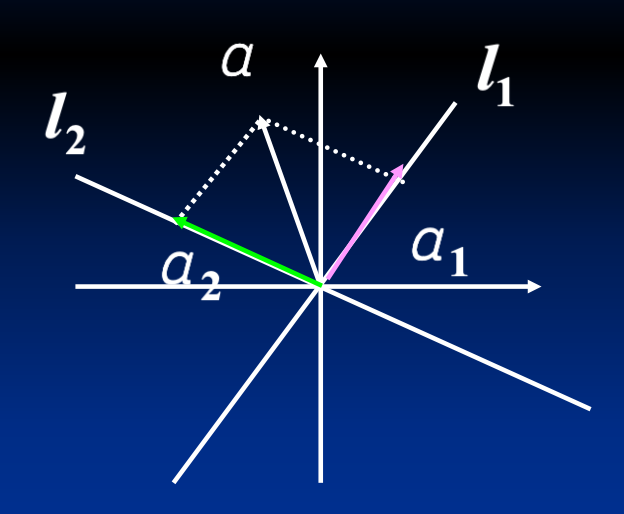
\includegraphics[scale=0.5]{直和分解——二维.png}
\end{figure}

在这个例子中,向量$\alpha$沿着两条直线$l_1,l_2$分解成了两个部分,这个时候,假设$l_1$是固定的,那么$l_2$就一定固定且唯一(可以画一个三角形,两条边都确定了那第三边一定也是确定的),那么这个时候就可以说$l_1+l_2$构成的二维空间是直和,二维空间的分解具有唯一性。

那事情到了三维空间,还是一样的吗?
\begin{figure}[h]
    \centering
    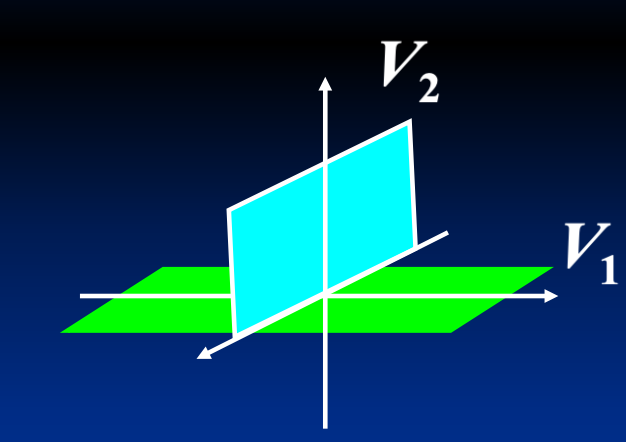
\includegraphics[scale=0.3]{直和分解——三维.png}
\end{figure}

在三维空间中,假设有一个向量$\alpha$,在$\V_1$中的分量,那他在$\V_2$中的分量会有无数种,这就是说,三维空间的分解不具有唯一性。

如果只利用直和的定义来判断直和是否成立有些太过麻烦,下面的定理能够方便我们判断直和:
\begin{them}{}{}
    设$\V_1, \V_2$是线性空间$\V$的子空间,则下列命题等价:
    \begin{enumerate}
        \item $\V_1+\V_2$是直和
        \item 零向量的表示方法唯一
        \item $\V_1\cap\V_2=\{\bs{0}\}$
    \end{enumerate}
\end{them}

也就是说,如果两个空间没有相同的部分,那它们的和一定是直和,分解出的基向量也一定没有相同的,维数也就等于两个空间各自维数之和。这就类似于两个互不相交的集合,他们的和可以类比为空间的“直和”。

前面所讲述的是两个空间内的直和,接下来给出一般情况下的直和及其性质:
\begin{defn}{}{}
    设$\V_1,\V_2,\cdots,\V_s$是线性空间$\V$的子空间,如果和$\V_1+\V_2+\cdots+\V_s$中的每个向量$\alpha$的分解式\[\alpha=\alpha_1+\alpha_2+\cdots+\alpha_s, \alpha_i\in\V_i\ \ \ (i=1,2,\cdots,s)\]是唯一的,这个和$\V_1+\V_2+\cdots+\V_s$就称为直和,记为\[\V_1\oplus\V_2\oplus\cdots\oplus\V_s\]
\end{defn}

\begin{them}{}{}
    设$\V_1,\V_2,\cdots,\V_s$是线性空间$\V$的子空间,则下列命题相互等价:


    \begin{enumerate}
        \item $\bs{W}=\V_1+\V_2+\cdots+\V_s$是直和
        \item 零向量的表示方法唯一
        \item $\V_i\cap(\sum_{j\neq i}\V_j)=\{\bs{0}\}$
        \item $\dim(\bs{W})=\sum\dim(\V_i)$
    \end{enumerate}
\end{them}

\section{特征值与特征向量}
本节课的内容虽然叫做“特征值与特征向量”,但内容并不只是简单的线性代数中介绍的特征值与特征向量,我们要更加深入理解特征值与特征向量这两个概念。
\subsection{内容回顾}
\subsubsection{特征值与特征向量}
先来回顾一下线性代数中学到的特征值与特征向量:
\begin{defn}{}{}
    设$\A\in\mathbb{P}^{n\times n}, \alpha\in\mathbb{P}^n, \lambda\in\mathbb{P}$,若\[\A\alpha=\lambda\alpha\ (\alpha\neq 0)\]则称$\lambda$为$\A$的一个\textbf{特征值},$\alpha$为$\A$对应于$\lambda$的一个\textbf{特征向量}。
\end{defn}

特征向量具有下面的性质:
\begin{enumerate}[leftmargin=4em]
    \item 设$\A\alpha=\lambda\alpha\ (\alpha\neq 0)$,则\[\A(k\alpha)=k(\A\alpha)=k(\lambda\alpha)=\lambda(k\alpha)\]
    \item 设$\A\alpha_i=\lambda\alpha_i\ (i=1,2,\cdots,s)$,则\[\A(k_1\alpha_1+k_2\alpha_2+\cdots+k_s\alpha_s)=\lambda(k_1\alpha_1+k_2\alpha_2+\cdots+k_s\alpha_s)\]
\end{enumerate}

\subsubsection{特征子空间}
对于所有的特征向量$\alpha$,设$\V_{\lambda}=\{\alpha|\A\alpha=\lambda\alpha, \alpha\in\R^n\}$,由特征值和特征向量的性质可知:
\[\forall\alpha,\beta\in\V_{\lambda}, \alpha+\beta\in\V_{\lambda}\ \ \text{(加法封闭)}\]
\[\forall\alpha\in\V_{\lambda},k\in\R,k\alpha\in\V_{\lambda}\ \ \text{(数乘封闭)}\]

因此,可以把$\V_{\lambda}$称作一个空间,这个空间叫做$\A$的\textbf{特征子空间}。

\subsection{谱、几何重数和代数重数}
回顾了已经学过的知识之后,接下来就是新内容了,首先介绍几个基本概念
\begin{defn}{}{}
    $\A$的所有特征值的全体称为$\A$的\textbf{谱},记为$\lambda(\A)$。
\end{defn}
\begin{defn}{}{}
    我们把
    \[|\lambda\bs{E}-\bs{A}|=(\lambda-\lambda_1)^{n_1}\cdots(\lambda-\lambda_r)^{n_r}\]叫做$\A$的特征多项式,$\sum\limits_{i=1}^{r}n_i=n$,这里$n_i$叫做特征值$\lambda_i$的\textbf{代数重数}。
    
    如果\[\rank(\lambda_i\bs{E}-\bs{A})=n-m_i\]$m_i$叫做$\lambda_i$的\textbf{几何重数}。
\end{defn}

几何重数与代数重数与后面Jordan标准型的内容紧密相关,代数重数就是特征方程中,该特征值的次数,几何重数与该特征值对应特征向量的特征矩阵的秩紧密相关。

\subsection{对角化与Jordan标准型}
在线性代数中,我们学过对一个矩阵进行相似对角化,了解了其步骤,并且了解能对一个矩阵进行相似对角化的条件。可现实中,能够对角化的矩阵毕竟是少数,将对角化的概念一般化,就是马上就要介绍的Jordan标准型。

\subsubsection{Jordan块与Jordan标准型}
\begin{them}{}{}
    设$\A\subseteq \C^{n\times n}$有$r$个不同的特征值:$\lambda_1, \lambda_2, \cdots,\lambda_r$, 其代数重数分别为$n_1, n_2,\cdots,n_r$,则必存在可逆矩阵$\P\in\C^{n\times n}$,使得\[\P^{-1}\A\P=\J=diag(\J_1(\lambda_1),\cdots,\J_r(\lambda_r))\]其中,矩阵$\J$叫做$\A$的Jordan标准型,$\J_1(\lambda_1),\cdots,\J_r(\lambda_r)$,叫做一个Jordan块,其结构为\[\J_i(\lambda_i)=\begin{bmatrix}
    \lambda_i&1&&\\
    &\lambda_i&1&\\
    &&\ddots&1\\
    &&&\lambda_i
    \end{bmatrix}\]
\end{them}

Jordan标准型有下面的几个结论(\textbf{一定要记住}):
\begin{enumerate}[leftmargin=4em]
    \item Jordan块的个数$k$是线性无关特征向量的个数
    \item 当且仅当$k=n$的时候矩阵可以对角化
    \item 一个已知特征值的Jordan块个数是该特征值的几何重数,同时也是相应特征子空间的维数,一个已知特征值的Jordan块的阶数之和是该特征值的代数重数。
    \item 特征值的几何重数小于等于其代数重数
    \item 矩阵不同特征值对应的特征向量线性无关
\end{enumerate}

那Jordan标准型和矩阵对角化有什么样的关系呢?看下面的定理:
\begin{them}{}{}
    设$\A\subseteq \C^{n\times n}$,则下列命题等价:
    \begin{itemize}
        \item $\A$是可对角化矩阵
        \item $\C^n$存在由$\A$的特征向量构成的一组基
        \item $\A$的Jordan标准型中的Jordan块都是一阶的
        \item $m_i=n_i\ (i=1,2,\cdots,r)$(代数重数=几何重数)
    \end{itemize}
\end{them}
\subsection{特征值与特征向量的几何性质}
\subsubsection{从线性变换开始说起}
我们将线性空间到自身的映射称之为\textbf{变换},如果在空间$\V$中存在变换$T$,并且满足\begin{enumerate}
    \item $\forall\alpha,\beta\in\V, T(\alpha+\beta)=T(\alpha)+T(\beta)$
    \item $\forall k\in \mathbb{P}, T(k\alpha)=kT(\alpha)$
\end{enumerate}

那么就成$T$是$\V$的\textbf{线性变换}。
\subsubsection{线性变换的特征值}
从纯数值上理解了特征值之后,接下来换一个角度,从线性变换的角度理解特征值与特征向量:
\begin{defn}{}{}
    设$T$是线性空间$V_n(C)$的一个线性变换,如果存在$\lambda\in\C$和非零向量$\xi\in\V_n(C)$,使得$T\xi=\lambda\xi$,则$\lambda$叫做$T$的特征值,$\xi$叫做$T$的属于特征值$\lambda$的特征向量。
\end{defn}

那这个线性变换的$T$与最开始从数值角度分析的特征值与特征向量的矩阵$\A$有何关系呢?下面推导一下。

\subsubsection{线性变换与矩阵}
我们假设$\V$是$n$维空间,$\varepsilon_1, \varepsilon_2,\cdots,\varepsilon_n$为该空间下的基,$T$为$\V$上的线性变换,则有\[T\varepsilon_1=\sum_{i=1}^{n}a_{i1}\varepsilon_i,\  T\varepsilon_2=\sum_{i=1}^{n}a_{i2}\varepsilon_2,\ \cdots,\ T\varepsilon_n=\sum_{i=1}^{n}a_{in}\varepsilon_n\]则有
\[\begin{aligned}
    T(\varepsilon_1,\varepsilon_2,\cdots,\varepsilon_n)&=(T\varepsilon_1,T\varepsilon_2,\cdots,T\varepsilon_n)\\
    &=(\varepsilon_1, \varepsilon_2,\cdots,\varepsilon_n)\begin{bmatrix}
        a_{11}&a_{12}&\cdots&a_{1n}\\
        a_{21}&a_{22}&\cdots&a_{2n}\\
        \vdots&\vdots&&\vdots\\
        a_{n1}&a_{n2}&\cdots&a_{nn}
    \end{bmatrix}\\
    &=(\varepsilon_1,\varepsilon_2,\cdots,\varepsilon_n)\A
\end{aligned}\]

这里的矩阵$\A$称为线性变换$T$在基$\varepsilon_1, \varepsilon_2,\cdots,\varepsilon_n$下的\textbf{矩阵}。

由此,我们从向量方程$T\xi=\lambda\xi$推出了矩阵方程$\A\x=\lambda\x$,反之,给定一个矩阵$\A$,也可以得出,在基底$\varepsilon_1, \varepsilon_2,\cdots,\varepsilon_n$下存在唯一的线性变换$T$与之对应。

\section{初等矩阵、酉矩阵和酉变换}
“初等矩阵”这个概念,我们在线性代数中学到过,可在这里,“初等矩阵”说的是:
\begin{defn}{}{}
    设$u,v\in\C^n,\sigma\in\C$,称\[\bs{E}(u,v,\sigma)=\bs{E}-\sigma \bs{uv}^H\]为初等矩阵
\end{defn}
在这里,我们把线性代数中的“初等矩阵”更名为“初等变换矩阵”。
\begin{itemize}
    \item $\bs{E}_{ij}=\bs{E}-(e_i-e_j)(e_i-e_j)^T=\bs{E}(e_i-e_j,e_i-e_j,1)$
    \item $\bs{E}_{ij}(k)=\bs{E}+ke_je_i^T=\bs{E}(e_j,e_i,-k)$
    \item $\bs{E}_i(k)=\bs{E}-(1-k)e_ie_i^T=\bs{E}(e_i,e_i,1-k)$
\end{itemize}
\subsection{初等矩阵的相关性质}
接下来介绍初等矩阵的相关性质,具体的证明过程都省略掉了(不想写证明过程了),感兴趣的可以翻看课本。
\subsubsection{初等矩阵的特征向量}
\begin{itemize}
    \item 当$u\perp v$时,设$u_1,u_2,\cdots,u_{n-1}$是与$u$垂直的空间(正交补子空间)的一组基,他们也是$\bs{E}(u,v,\sigma)$的$n-1$个线性无关的特征向量。
    \item 若$u$不与$v$垂直时,设$u_1,u_2,\cdots,u_{n-1}$是与$u$垂直的空间(正交补子空间)的一组基,则$u, u_!,\cdots,u_{n-1}$是$\bs{E}$的$n$个无关特征向量。
\end{itemize}

\subsubsection{初等矩阵的特征值}
\[\lambda(\bs{E}(u,v,\sigma))=\{1,1,\cdots,1,1-\sigma v^Hu\}\]
\subsubsection{初等矩阵的行列式}
\[\det(\bs{E}(u,v,\sigma))=1-\sigma v^Hu\]
\subsubsection{初等矩阵的逆}
\[\bs{E}(u,v,\sigma)^{-1}=\bs{E}(u,v,\frac{\sigma}{\sigma v^Hu-1}),\ (1-\sigma v^Hu\neq 0)\]
\subsubsection{其他性质}
非零向量$a,b,\in\C^n$,存在$u,v,\sigma$,使得\[\bs{E}(u,v,\sigma)a=b,\ (\sigma u=\frac{a-b}{v^Ha})\]
\subsection{初等下三角阵}
\begin{defn}{}{}
    \[L_i(l_i)=\bs{E}(l_i,e_i,1)=\begin{bmatrix}
        1&&&&&&\\
        &\ddots&&&&\\
        &&1&&&&\\
        &&-l_{i+1,i}&\ddots&&\\
        &&\vdots&&1&\\
        &&-l_{n,i}&&&1
    \end{bmatrix}\]
其中

\[\begin{cases}
    l_i=(0,\cdots,0,l_{i+1},\cdots,l_{n,i})^T\\
    e_i=(0,\cdots,0,1,0,\cdots,0)^T
\end{cases}\]

\[l_{k,i}=\frac{a_{k,i}}{a_{i,i}}(k=i+1,\cdots,n), \bs{E}(l_i,e_i,1)\A=\overset{\sim}{\A}\Rightarrow \overset{\sim}{a}_{k,i}=0\ (k=i+1,\cdots,n)\]
\end{defn}

\subsection{初等酉阵(Householder变换)}
\begin{defn}{}{}
    \[\H(u)=\bs{E}(u,u;2)=\bs{E}-2uu^H,\ (u^Hu=1)\]
    \begin{enumerate}
        \item $\H(u)^H=\H(u)-\H(u)^{-1}$
        \item $\H(u)(a+ru)=a-ru,\ \forall a\in u^{\perp}, r\in\C$(镜像变换)
    \end{enumerate}
\end{defn}
\section{欧式空间上的度量}
本节只介绍相关的定理和性质,不涉及具体证明,本节内容无非就是将之前所学过的熟知的一些性质放到向量空间中罢了。
\begin{defn}{}{}
    在线性空间$\V_n(\P)$上,若映射
\end{defn}
\section{酉空间的分解与投影}
\ifx\allfiles\undefined
\end{document}
\fi